\section{Analysis}
In this section we will illustrate the scenario on which we have tested our tool, traffic analysis is mainly based on IP addresses and timestamp\cite{ddos_forensics}.More over we will show two examples of attack, DDoS and DoS, in order to explain and evaluate our analysis quality trying to base our conclusion by using different datasets\footnote{Mentioned dataset were generated by our tool, it is possible to analyse every type of dataset on your own if in \texttt{pcap} format.}. There is also a summary of how to configure and run an analysis with \textit{Python} and \textit{Hadoop}.


\subsection{Configuring and Running Analysis}
This tool has been developed for running analysis over network flow records with minimal effort from the user. Once installed and configured \textit{Hadoop} on your PC or cluster, only one line of code is needed for running and storing the results of an analysis, as shown in the example below

\begin{lstlisting}[firstline=1, lastline=1]
   python3 DDoSAnalysis.py -a dataset_name
	Write('Case insensitive '); 
	Write('Bash keywords.')
\end{lstlisting}

\subsection{Scenario} 
The scenario we focusing on is illustrated in fig.\ref{fig:networkscenario}, as we can see it is a very simple and basic design scenario. There is a \textit{router} that communicates with \textit{internet},  it connects the \textit{sever} with the global network, as we will see further on the treatment \textit{internet} may contains one or several attackers which aim is to deny the service give by the \textit{server}. 

In this scene common users exchange with the server at least 650 MB, the upper bound is $800$ MB with an average speed of $2.2$ Kb/s during the user server connection lifecycle. These data comes from an analysis in normal\footnote{Dataset generated without attackers in order to get an estimation of normal traffic conditions.} server condition, these assumptions are based on a \textit{log} file with a pool of one hundred users. As we will se further this assumption is the ground truth for our analysis under attacks condition.

We choose this type of network configuration in order to concentrate our heed on the implementation of analysis tools and big data scripting, which are the main topics of this project.
  
\subsection{DoS Analysis Example}
A DoS attack is a common way to saturate the server bandwidth. It's often used in combination with other vulnerabilities to amplificate the DoS traffic volume, as we have seen in the wild with the Memcached vulnerability\cite{memcached_vulnerability}. In our example, fig. \ref{fig:DoS}, we don't consider the possibility to track the real culprit behind a proxy.
In our PoC we generated a dataset with the configuration in Table \ref{tab:tab:dos_config} and we started our analysis.

\begin{table}[h]
\centering
\begin{tabular}{|l|c|}
\hline
\textbf{Parameter} & \textbf{Value} \\ \hline
 Number of users & 100 \\ 
 Number of lines & 20000000 \\ 
 Number of attackers & 1 \\ 
 Attack volume & 1 Gbit \\
 Attack duration & 1 second \\  
 \hline 
\end{tabular}
\caption{DoS configuration}
\label{tab:tab:dos_config}
\end{table}

We can immediately see in fig. \ref{fig:dos_analysis} how the attacker with \textit{id 0} is immediately recognized because of a small amount of traffic volume compared to a large spike in packet speed. Here, in the two graphs, we can see the mean value, represented in a red line: the attacker squared root margin from the sigma value is also more accentuated in both graphs, which suggests an involvement in the DoS genesis.

\subsection{DDoS Analysis Example}
DDoS is a popular approach for attackers to paralyse computers or network systems by coordinating flooding traffic originated from multiple hosts simultaneously, to block legitimate users' system access by reducing resource availability. DDoS attack inherits similar characteristics of DoS attacks, with the differences in an increased scale which in term yields a higher impact\cite{ddos_forensics}.

In our attack scenario, fig. \ref{fig:DDoS},  the attacker controls a botnet of forty devices capable to generate a traffic volume to our server of 1 GB/s. By using \textit{UDP flood} attack the botmaster unleash his botnet against the server for four seconds overwhelming it. Launching our analysis tool, thanks to its big data features, we are capable to deal with the \texttt{ddos\_log} file easily.

The analysis results are shown in fig. \ref{fig:ddos_analysis}, as we can see there are two  visible clusters, one of legitimate users and one of attacker. We can easily recognise attackers from legitimate users because the data exchanged in terms of KB is very low (fig. \ref{fig:ddos_data}) but on the other hand volume of data exchanged in therms of KB over seconds are high respect the average of norma traffic on the server in normal conditions. Our tool output also a dataset which contains the IP and all the statistics previously mentioned, in this dataset we can retrive the ip of the attacker by its id which is used to identify it into the output figures. 

\begin{figure*}[h]
	\begin{subfigure}{0.48\textwidth}
		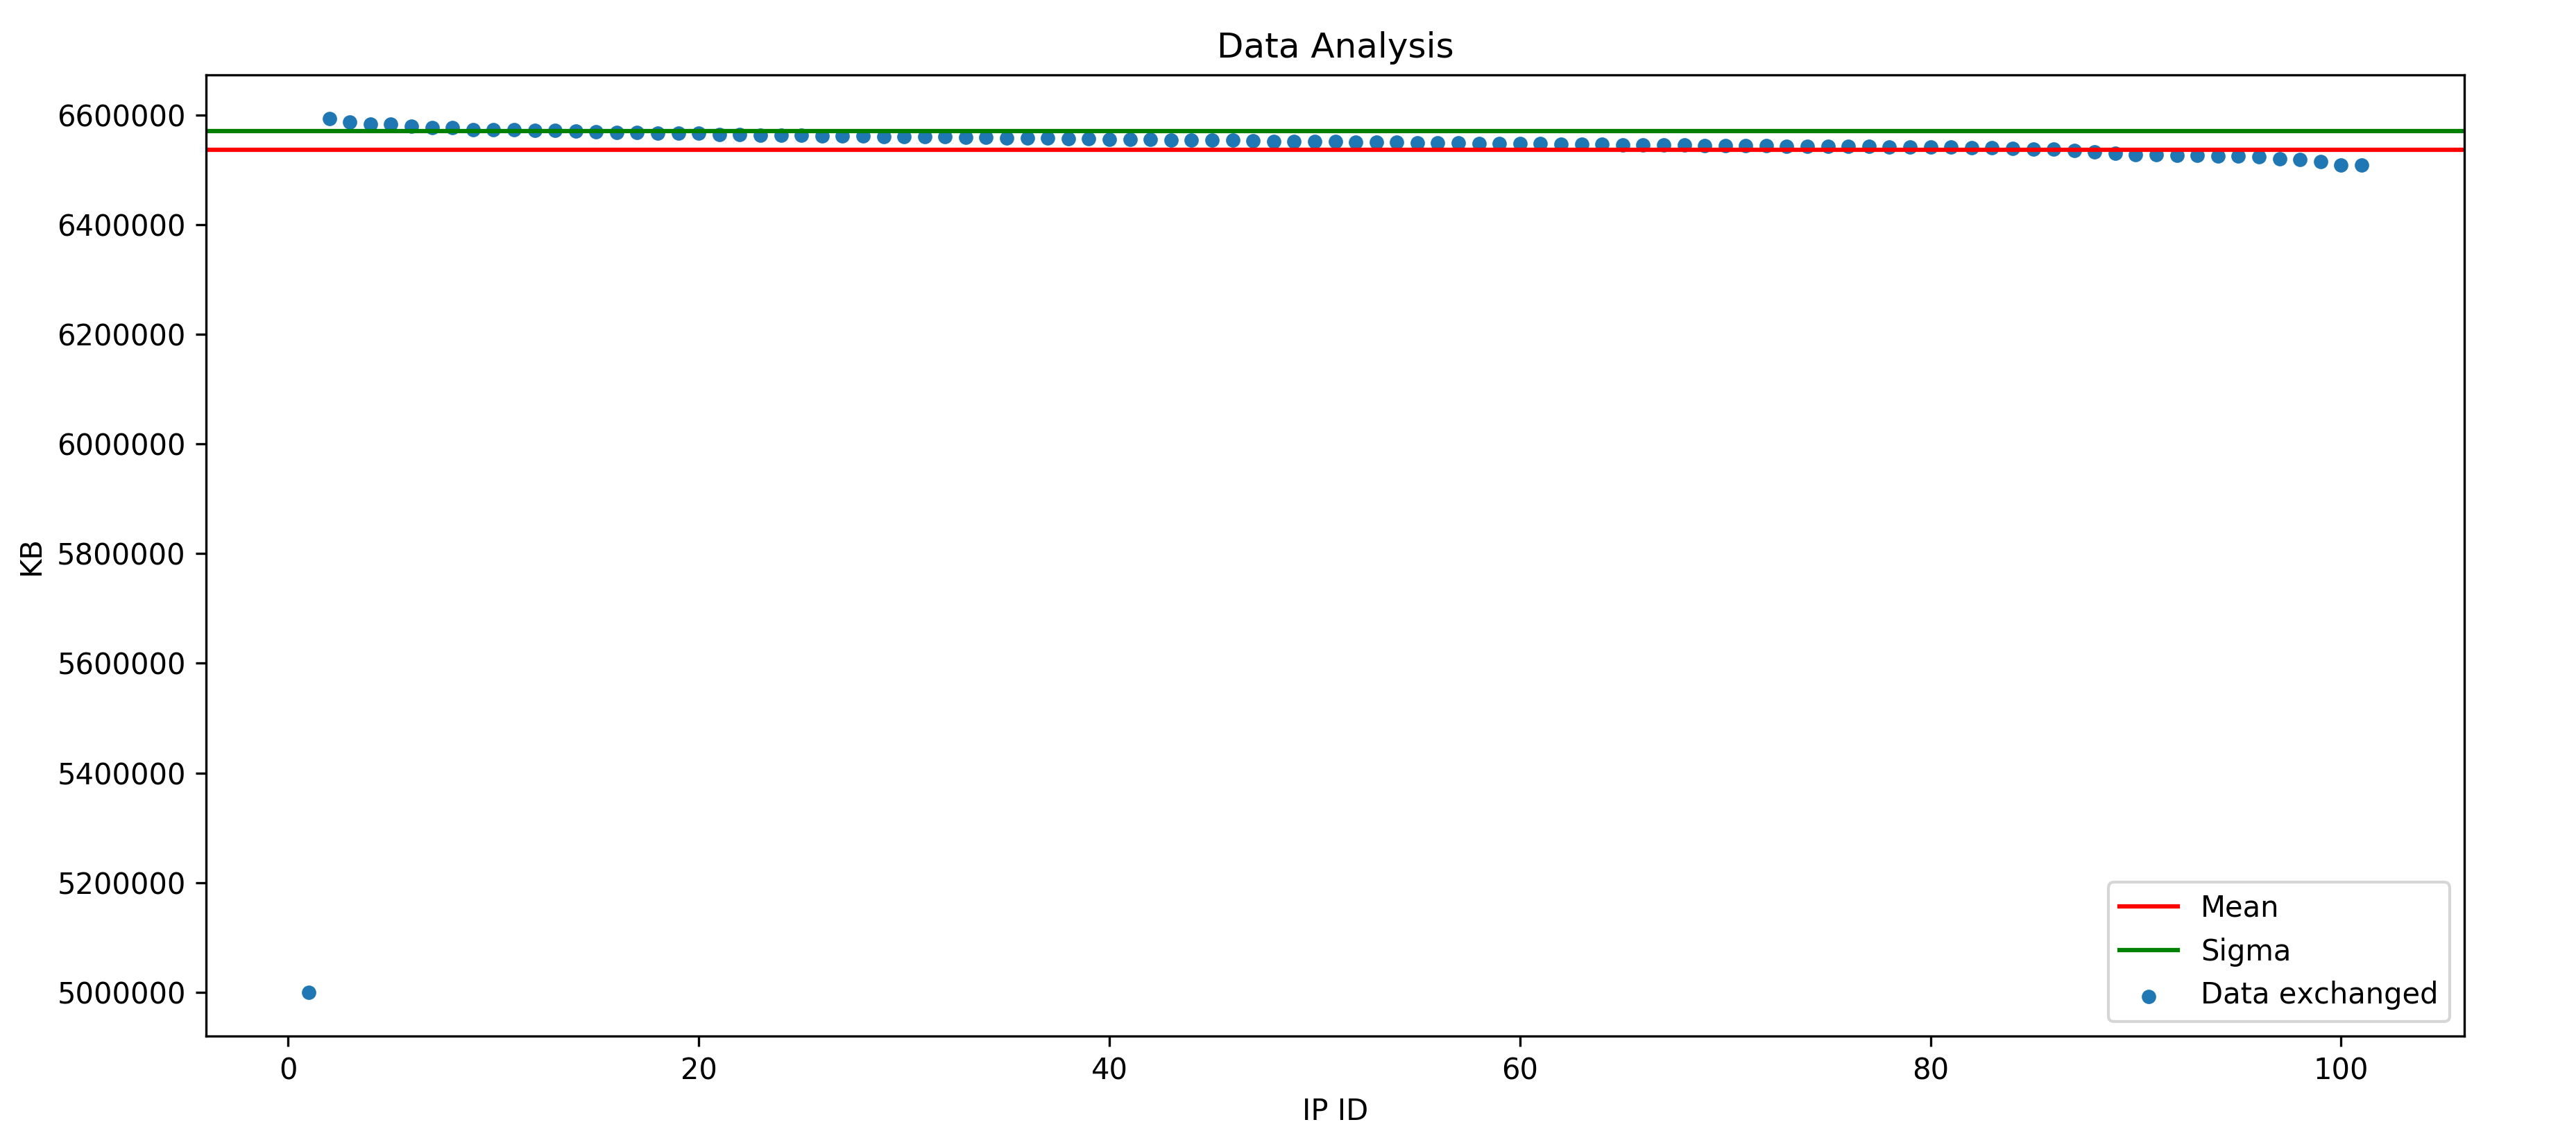
\includegraphics[width=\textwidth]{imgs/dos_atk-data_analysis.png}
  		\caption{DoS Data Analysis}
  		\label{fig:ddos_data}
	\end{subfigure}
	\hspace*{\fill} % separation between the subfigures
	\begin{subfigure}{0.48\textwidth}
  		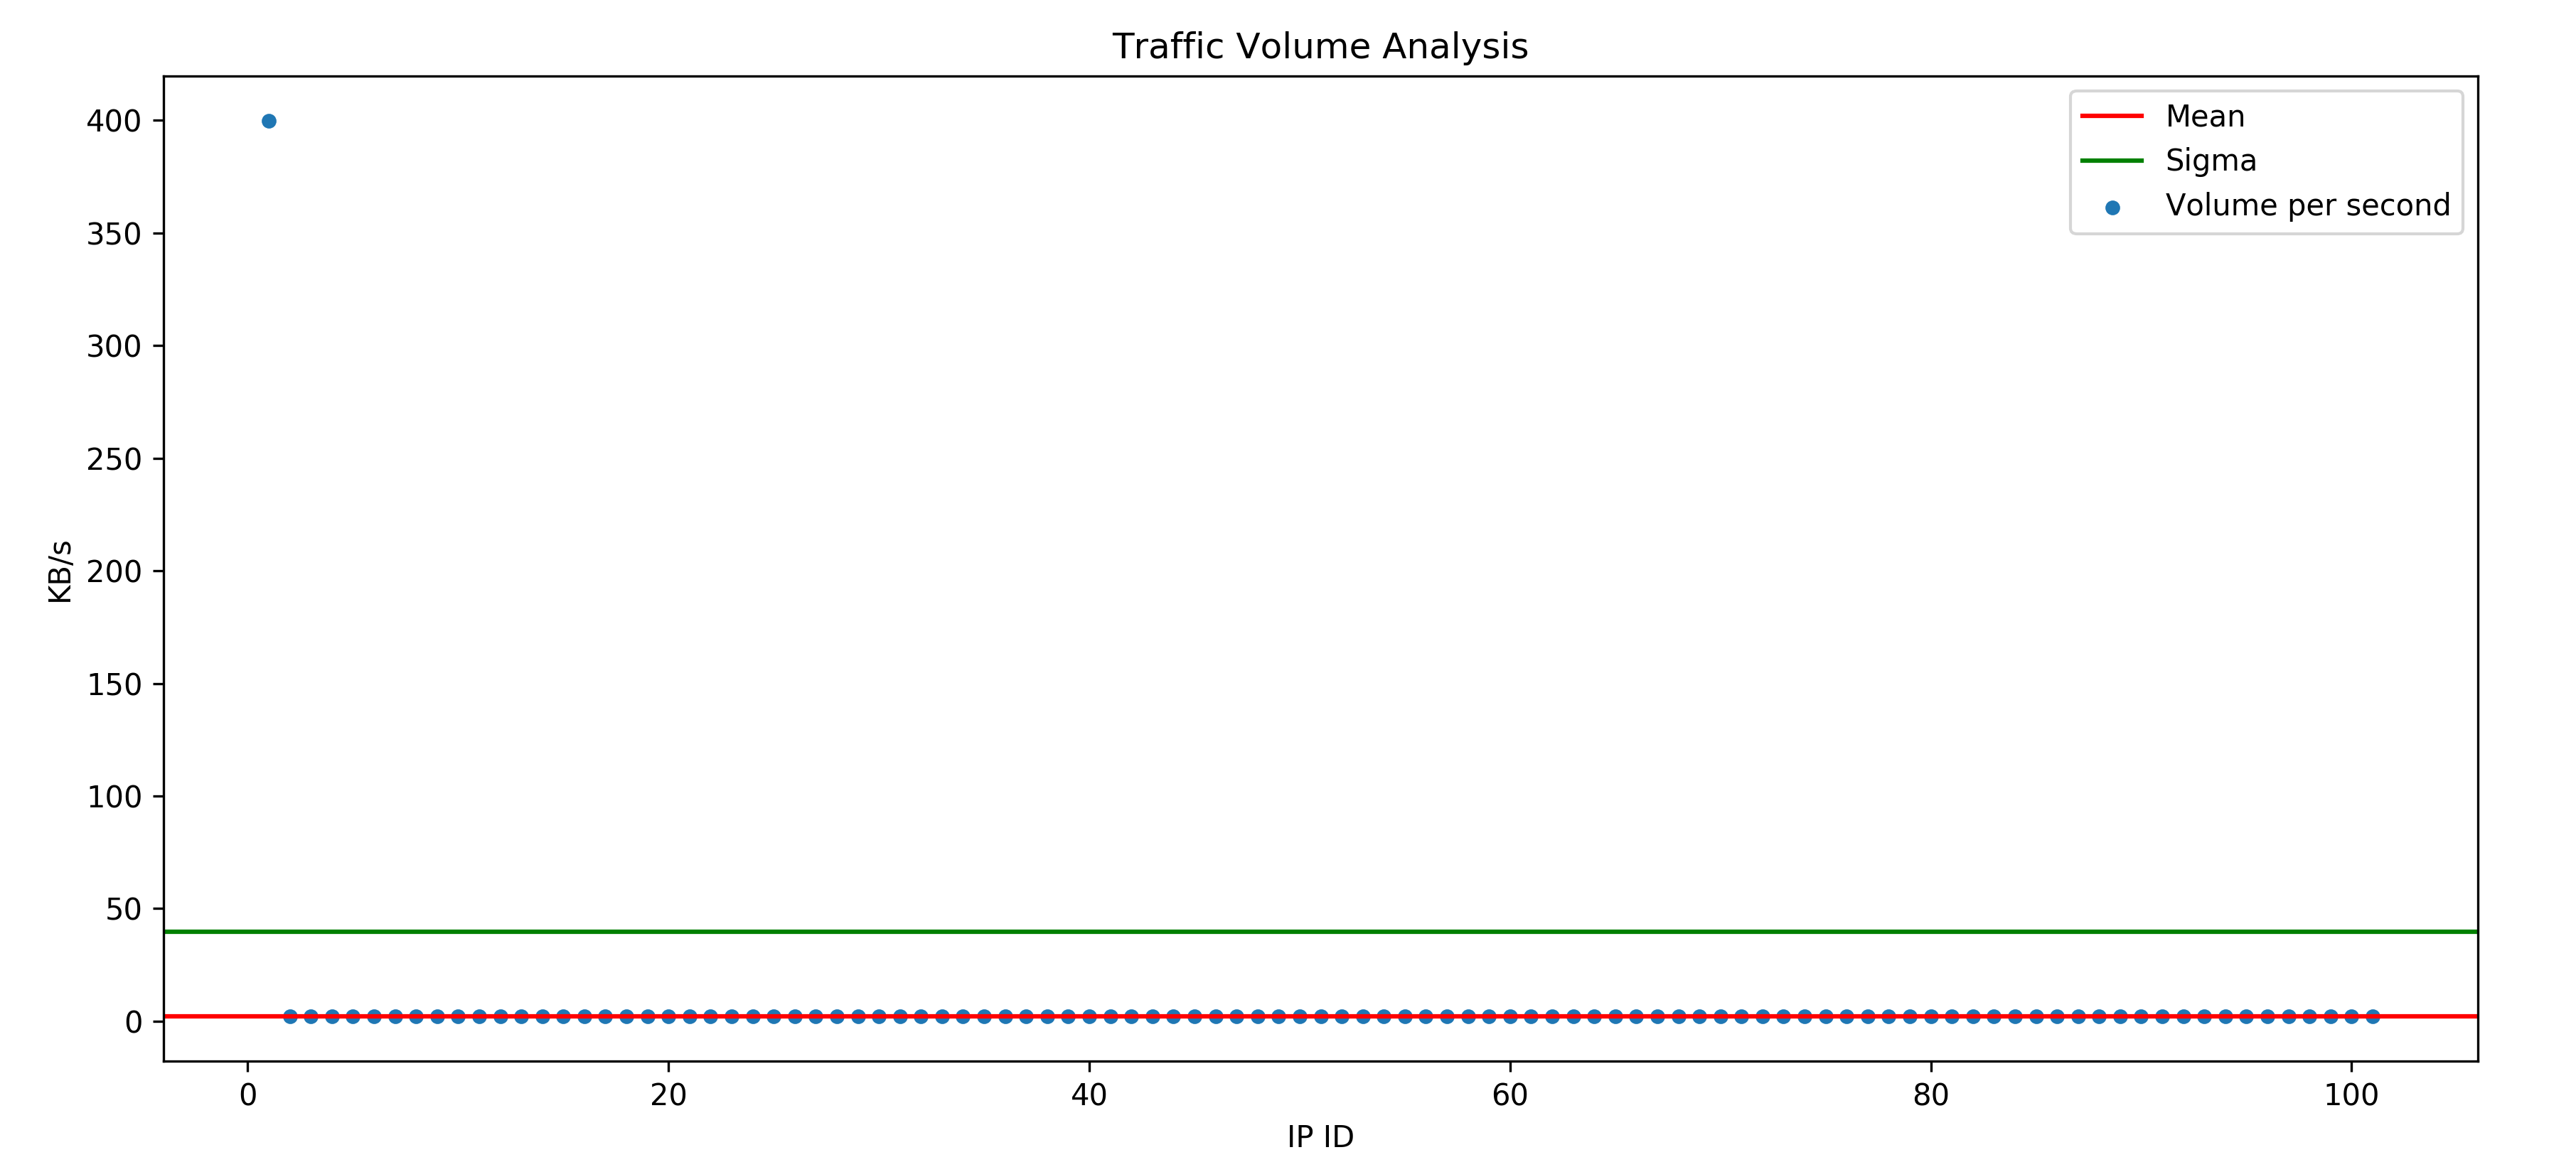
\includegraphics[width=\textwidth]{imgs/dos_atk-volume_analysis.png}
  		\caption{DoS Volume Analysis}
  		\label{fig:dos_volume}
	\end{subfigure}
	\caption{DoS attack Analysis}
	\label{fig:dos_analysis}
\end{figure*}

\begin{figure*}[h]
	\begin{subfigure}{0.48\textwidth}
		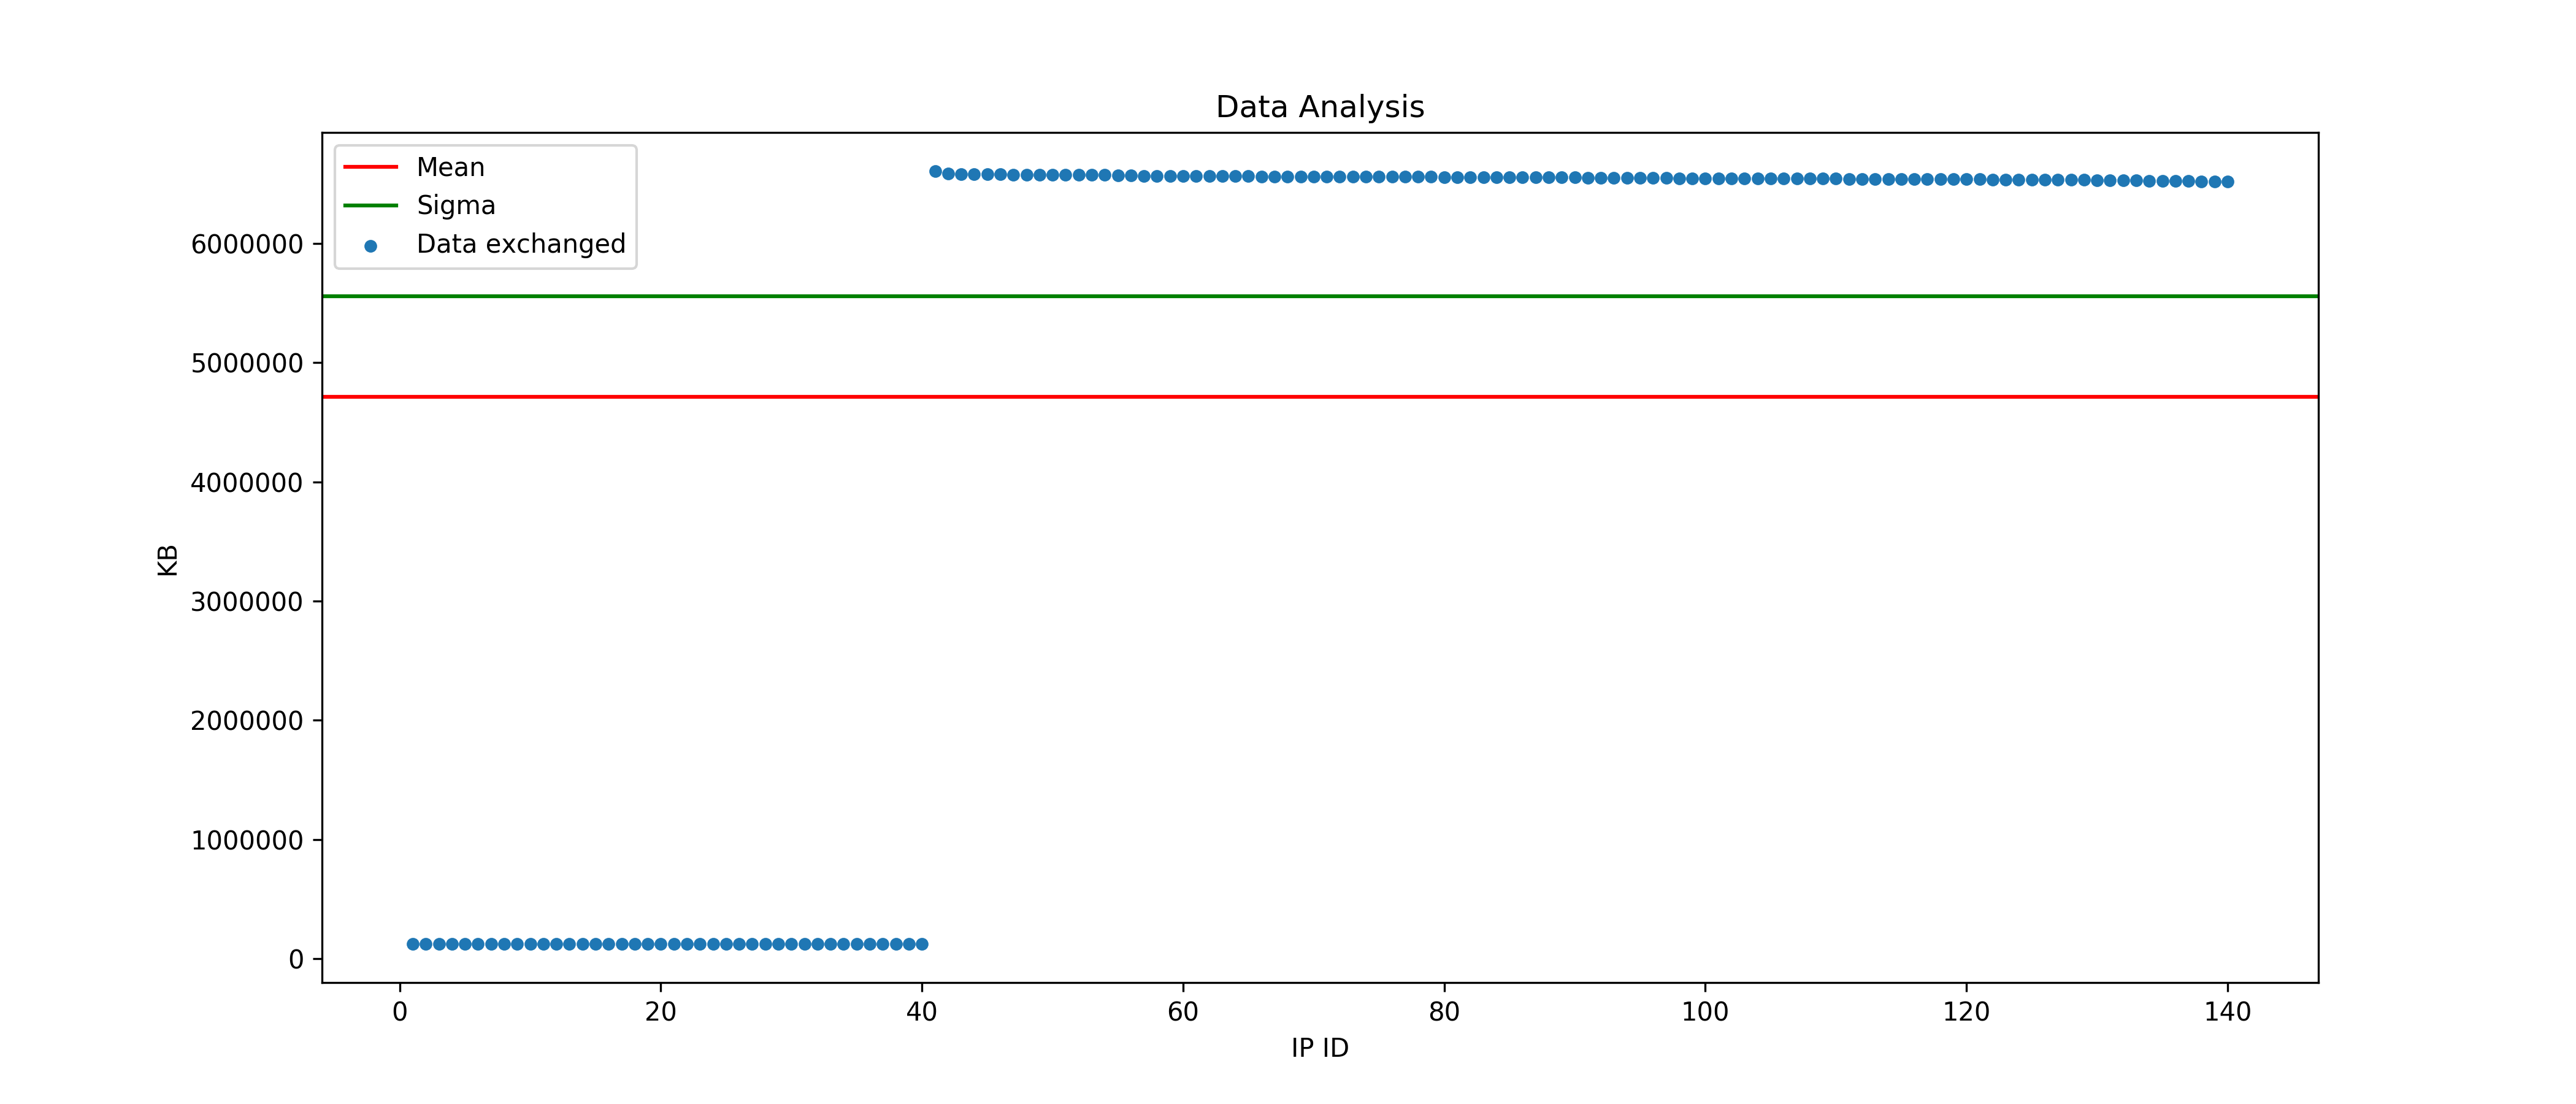
\includegraphics[width=\textwidth]{imgs/ddos_atk-data_analysis.png}
		\caption{DDoS Data Analysis} 
		\label{fig:ddos_data}
	\end{subfigure}
	\hspace*{\fill} % separation between the subfigures
	\begin{subfigure}{0.48\textwidth}
		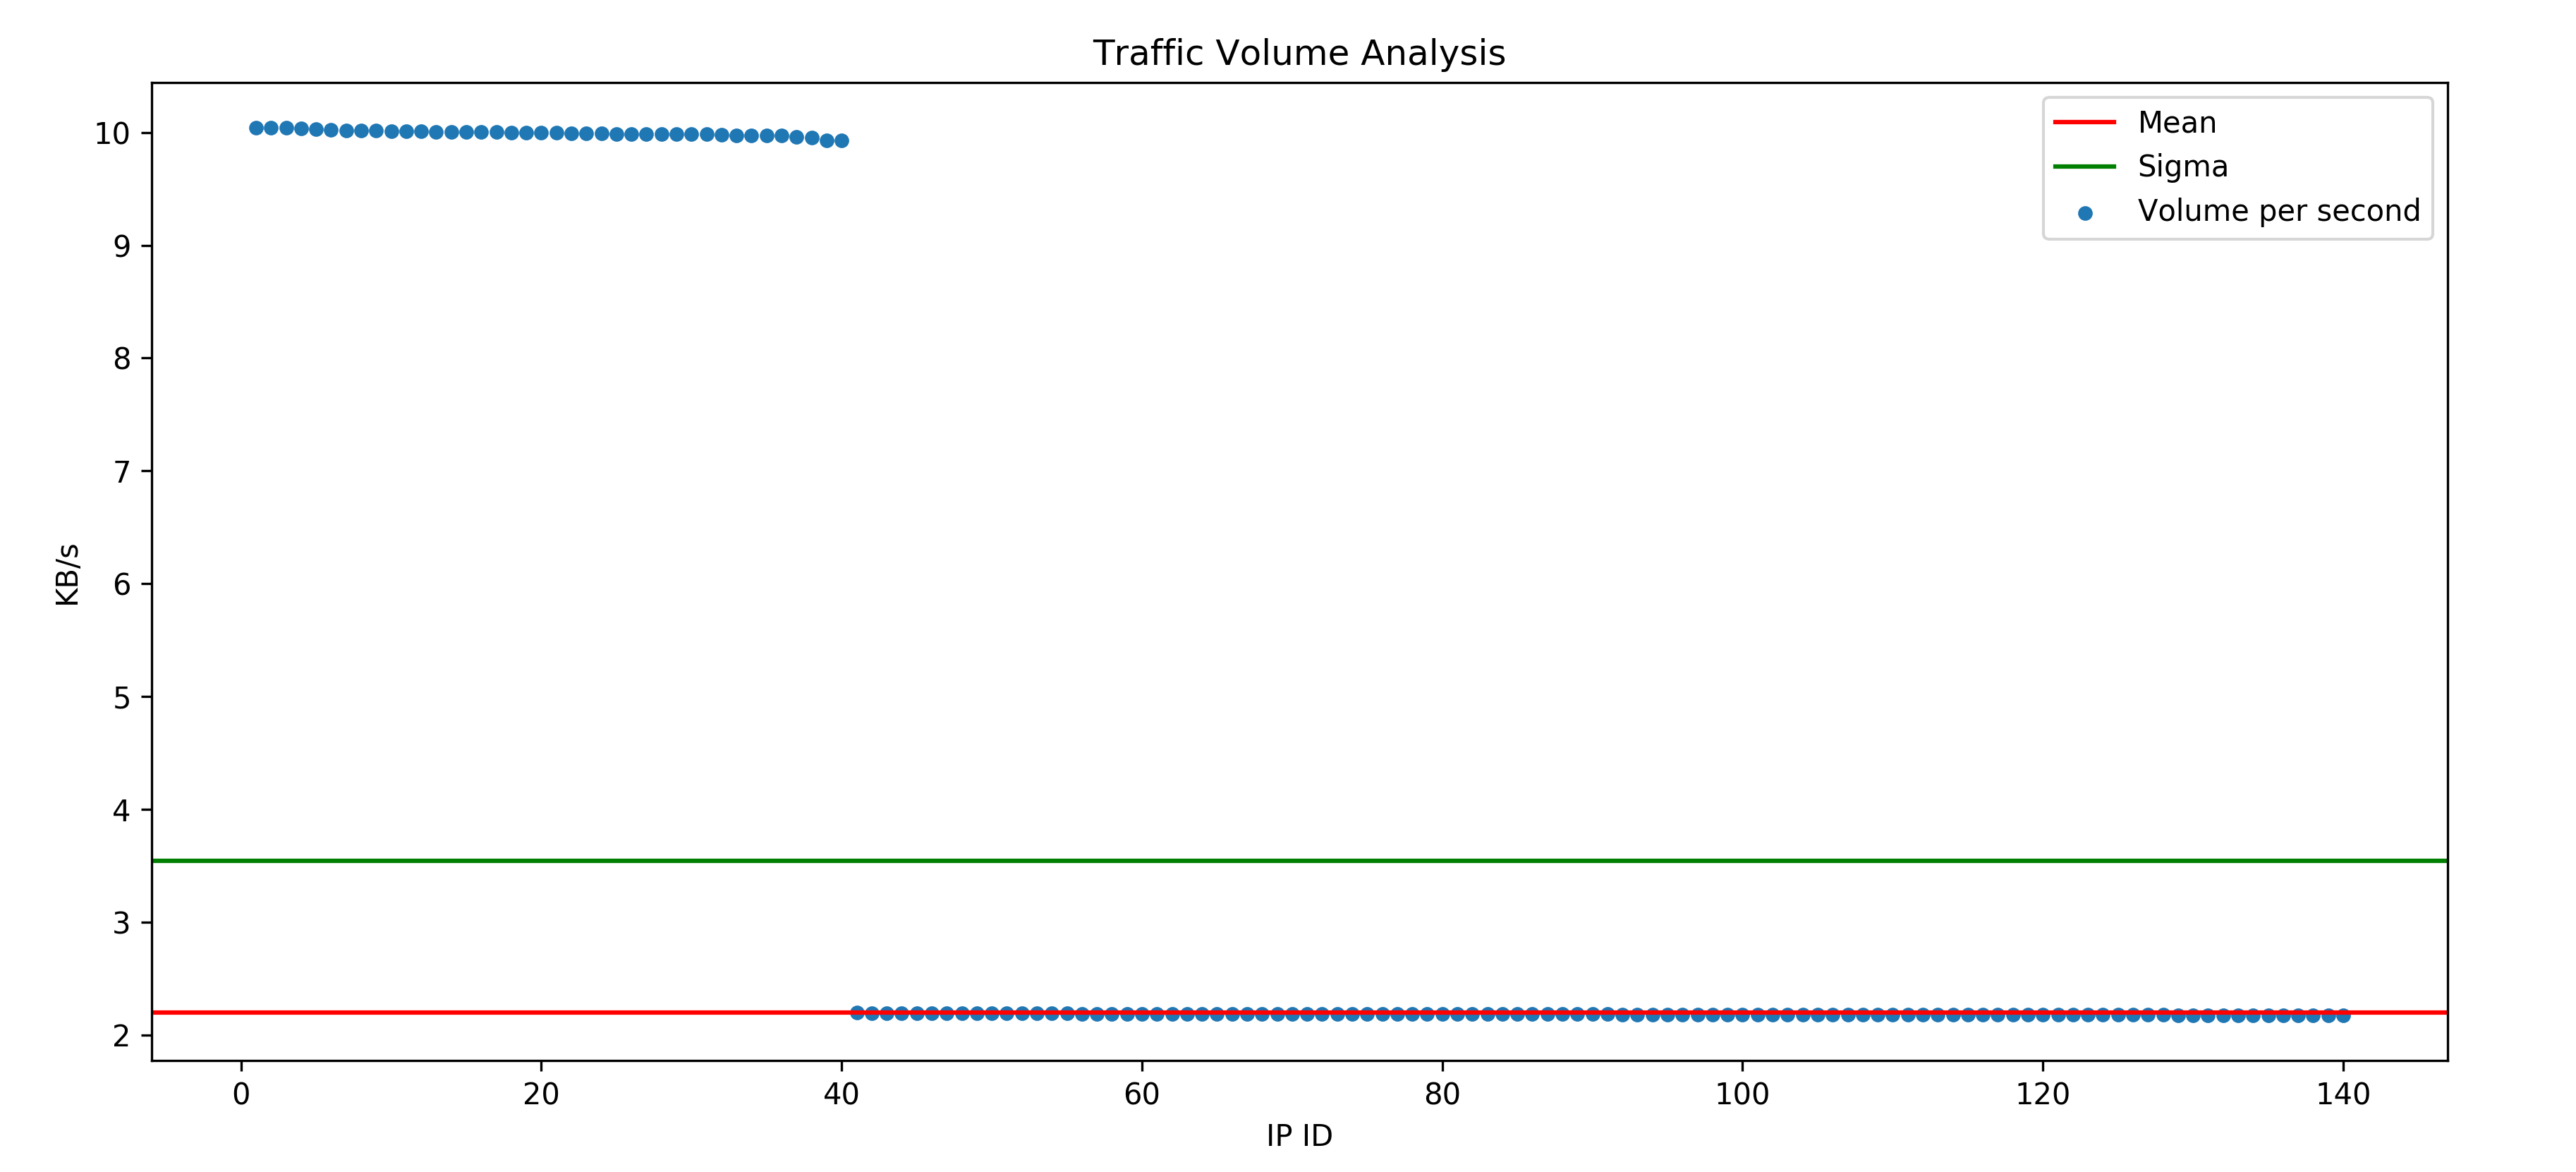
\includegraphics[width=\textwidth]{imgs/ddos_atk-volume_analysis.png}
		\caption{DDoS Volume Analysis} 
		\label{fig:ddos_volume}
	\end{subfigure}
	\caption{DDoS attack Analysis}
	\label{fig:ddos_analysis}
\end{figure*}
